\documentclass[border=5pt]{standalone}
\usepackage[utf8]{inputenc}
\usepackage{amssymb}
\usepackage{amsmath}
\usepackage{tikz}
\usetikzlibrary{arrows.meta}

\begin{document}
\nopagecolor
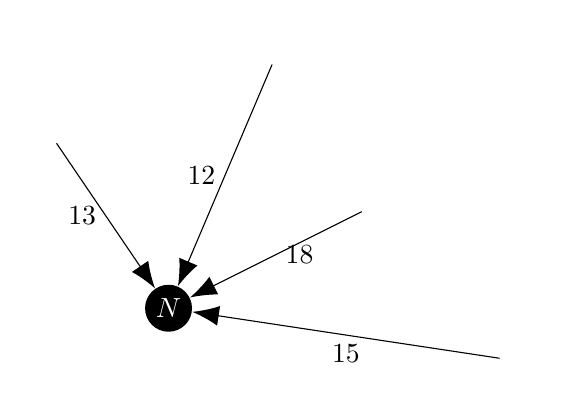
\begin{tikzpicture}
    \node (0) at (0, 0) {\color{white} 0};
    \node (1) at (-3, -1) {\color{white} 1};
    \node[circle, inner sep=2pt, fill] (N) at (-1.416, -3.333) {\color{white} $N$};
    \node (3) at (1.25, -2) {\color{white} 3};
    \node (7) at (3, -4) {\color{white} 7};

    \draw [-{Latex[scale=2]}] (0) -- node[left]{12} (N);
    \draw [-{Latex[scale=2]}] (1) -- node[left]{13} (N);
    \draw [-{Latex[scale=2]}] (3) -- node[right]{18} (N);
    \draw [-{Latex[scale=2]}] (7) -- node[below]{15} (N);
    
\end{tikzpicture}
\end{document}